%
%

\documentclass[french]{cv-style}
\sethyphenation[]{french}{} %
\usepackage[final,factor=1100,stretch=10,shrink=10]{microtype}
\usepackage[hidelinks]{hyperref}
\usepackage{xcolor}
\usepackage{siunitx}
\usepackage{multirow}
\usepackage{calc}
%

\hypersetup{
  pdftitle=CV \textbar{} Corentin Cadiou,
  pdfauthor=Corentin Cadiou,
  pdfsubject=CV,
}
\usepackage{soul}
\setul{1.5pt}{.6pt}
\newcommand{\myhref}[2]{\href{#1}{%
  \setul{1pt}{.4pt}%
  \setulcolor{red}%
  \ul{#2}}%
}

\newcommand{\asterisk}{$\star$\hspace{-3pt}}
\newcommand{\highlight}[1]{\colorbox{verylightgray}{\textbf{#1}}}
\renewcommand{\hl}[1]{\textbf{\color{darkred}#1}}

%
\newcommand{\vcenteredinclude}[1]{\begingroup
\setbox0=\hbox{\includegraphics[height=1em]{#1}}%
\parbox{\wd0}{\box0}\endgroup}

\makeatother
\begin{document}
\header
{Corentin}
{Cadiou}
{Postdoc à University College London (UCL)}
%
%

%
%
%

\begin{aside}
~\vspace{0.9em}
\hfill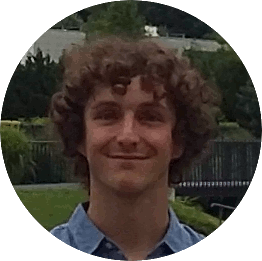
\includegraphics[width=.6\columnwidth]{inset.png}%
~\vspace{-0.5em}
%
\section{Contact}
\color{black}%
Department of Physics and Astronomy
University College London
WC1E 6BT Londres
Royaume-Uni
~\vspace{-0.8em}
\vcenteredinclude{images/at.pdf}\hfill\myhref{mailto:c.cadiou@ucl.ac.uk}{c.cadiou@ucl.ac.uk}
\vcenteredinclude{images/link.pdf}\hfill\myhref{https://cphyc.github.io/}{cphyc.github.io}
\vcenteredinclude{images/github.pdf}\hfill\myhref{https://github.com/cphyc}{github.com/cphyc}
\vcenteredinclude{images/orcid.pdf}\hfill\myhref{https://orcid.org/0000-0003-2285-0332}{orcid:0000-0003-2285-0332}
%
\section{Astrophysique}
formation des galaxies
toile cosmique
simulations
cosmologie
%
\section{Langues}
\hspace{-1em}Français: langue natale
Anglais: avancé
\hspace{-2em}(114/120 au TOEFL, 2016)
\hspace{-1em}Allemand: intermédiaire
%
\section{Programmation}
\vspace{-2.5em}~
\textbf{— Calcul haute perf. —}
RAMSES
MPI, OpenMP, Fortran, C++, OpenCL
~\vspace{-0.8em}
\hspace{-1em}\textbf{— Analyse de données —}
{\sc Yt}, pynbody, tangos
Python, Cython, Linux
~\vspace{-0.8em}
\textbf{— Divers —}
Linux, bash, javascript
\LaTeX
%
\end{aside}

%
%
%

\section{Expérience de recherche}
\begin{entrylist}
%
\entry
{2019 -- 2022}
{Assistant de recherche postdoctoral}
{University College London (UCL), Royaume-Uni}
{Travaux théoriques et numériques en collaboration avec A.~Pontzen et H.~V.~Peiris sur l'origine du moment angulaire des galaxies et de la matière noire.}
%
\entry
{2016 -- 2019}
{Doctorant}
{Institut d'Astrophysique de Paris (IAP), Paris, France}
{\emph{L'impact des grandes structures de l'Univers sur la formation des halos de matière noire et des galaxies}. Encadrants: C.~Pichon et Y.~Dubois, bourse: allocation spécifique normaliens.}
%
\entry
{2016}
{Kavli Summer Program}
{University of California Santa Cruz (UCSC), USA}
{École d'été prestigieuse de 6 semaines, travaux sur l'évolution de l'atmosphère des exoplanètes proches dans le catalogue Kepler, superviseurs: J.~Owen and F.~Adams.}
%
\entry
{2014}
{Stage de recherche de 6 mois}
{UCSC, USA}
{Travaux de simulation sur les processus de transport du moment angulaire dans les géantes rouges: une explication de l'origine des cœurs en rotation lente, superviseure: P.~Garaud.}
\end{entrylist}

\vspace{-1em}
\textbf{Participation à des collaborations}

\begin{entrylist}
  %
\entry
{2019 -- 2022}
{Membre du projet GMGalaxies}
{}
{ERC: \emph{l'origine de la diversité morphologique des galaxies à l'ère des grands relevés spectrographiques}, PI : A.~Pontzen.}
%
\entry
{2016 -- 2018}
{Membre du projet SPIN(E)}
{}
{ANR: \emph{L'origine cosmique de la séquence de Hubble}, PI : C.~Pichon.}
\end{entrylist}

\vspace{-1em}
\textbf{Articles revues rang A:}%
\begin{tabular}[t]{l}
  \hl{4 articles} en tant qu'auteur ou co-auteur principal (4 déjà publiés);\\
  \hl{7 articles} en tant que contributeur (5 déjà publiés);\\
  156 citations et h-index 6 (au \today); \href{https://ui.adsabs.harvard.edu/search/filter_database_fq_database=AND&filter_database_fq_database=database%3A%22astronomy%22&fq=%7B!type%3Daqp%20v%3D%24fq_database%7D&fq_database=(database%3A%22astronomy%22)&p_=0&q=((author%3A%22Cadiou%2C%20C%22))&sort=date%20desc%2C%20bibcode%20desc}{\setul{1pt}{.4pt}%
  \setulcolor{red}%
  \ul{source: NASA/ADS}}.
\end{tabular}

%
%
%

\section{Formation}

\begin{entrylist}
%
\entry
{2019}
{Thèse de doctorat}
{Sorbonne Université \& IAP, Paris, France}
{Rapporteurs: S.~White (MPA, Allemagne) et A.~Dekel (Hebrew University, Israël). Examinateurs: O.~Hahn, A.~Slyz, D.~Pogosyan et B.~Sémelin.}
%
\entry
{2016}
{Master 2 d'astronomie et d'astrophysique d'Île de France}
{Obs. de Paris, France}
{Spécialisation en cosmologie et astrophysique numérique, mention très bien.}

%
\entry
{2015}
{Diplôme de l'ENS}
{ENS, Paris, France}
{Majeure: physique, master 1 de physique théorique ICFP. Mineure: informatique.}
%
%
%
%
%
%
%
%
%
%
%
%
%
%
%
%
%
%
%
%
%
%
%
%
%

\end{entrylist}

%
%
%
\section{Demandes de temps de calcul}
J'ai participé à plusieurs demandes de temps de calcul sur les infrastructures britanniques (DiRAC) et françaises (CINES). Les équivalents financiers sont basés sur les équivalences des \myhref{https://www.genci.fr/sites/default/files/Modalitesdacces.pdf}{infrastructures du CINES}.
\begin{entrylist}
%
\entry
{2021}
{13\ieme{} appel à projet DiRAC -- projet \emph{Angular momentum genetic modifications}}
{}
{\hl{PI d'un projet} (8Mh de calcul \emph{demandées}, allocations attribuées en mars 2021, $\sim \SI{73}{k€}$) sur les infrastructures nationales britanniques (DiRAC).}
%
\entry
{2021}
{13\ieme{} appel à projet DiRAC -- projet EDGE 2.0}
{}
{Contribution au projet EDGE 2.0 (44Mh de calcul \emph{demandées}, allocations attribuées en mars 2021), PI: J.~Read (Surrey University).}
%
\entry
{2018 -- 2019}
{Allocation CINES}
{}
{Allocation de 17Mh (dont 2Mh pour projet personnel, $\sim \SI{18}{k€}$), PI: M.~Volonteri (IAP), sur les infrastructures nationales françaises (CINES).}
%
\entry
{2017 -- 2018}
{Allocation CINES}
{}
{Allocation de 11Mh (dont 2Mh pour projet personnel, $\sim \SI{18}{k€}$), PI: M.~Volonteri (IAP).}
\end{entrylist}

\section{Prix et bourses}
\begin{entrylist}
%
\entry
{2018}
{\emph{NumFOCUS New Contributor Award}}
{}
{Décerné pour ma contribution significative au développement et au support du code \textsc{Ramses} pour le projet \textsc{Yt}, une librairie en Python pour l'analyse et la visualisation de simulations astrophysiques (\myhref{https://numfocus.org/blog/inaugural-numfocus-awards-and-new-contributor-recognition}{lien}).}
%
\entry
{2017 --}
{Membre de l'équipe \textsc{Yt}}
{}
{Contribution au comité d'orientation du projet et à l'organisation de son développement (\myhref{https://yt-project.org/members.html}{lien}).}
%
\entry
{2016 -- 2019}
{Bourse de l'Institut Lagrange Paris (ILP)}
{}
{Allocation de 5000€/an pour les dépenses de recherche, dont les voyages (\myhref{http://ilp.upmc.fr/members-phdthesis-fr.php}{lien}).}
%
%
%
%
%
%
%
%
%
%
%
%
\end{entrylist}

%
%
%

%
%
%
%
%

%

%
%
%
%
%
%
%
%
%
%
%
%
%
%
%
%
%
%
%
%
%
%
%
%
%
%
%
%
%
%
%
%
%
%
%


%

%
%
%
%
%
%
%
%
%
%
%
%
%


%

%
%
%
%
%
%
%
%

%

%
%
%
\section{Présentations \& conférences}%

Les entrées marquées d'une étoile ont été décallées ou annulées du fait de la COVID-19.

\textbf{Invitation aux conférences}

\begin{entrylist}
  \entryshortnohl{01/2021}{LCDM -- Dark matter in Cosmology}{Londres, Royaume-Uni}
  \entryshortnohl{06/2020 \asterisk}{\textsc{Yt} Workshop}{ROE, Edimbourg, Royaume-Uni}
  \entryshortnohl{10/2019}{Yonsei-IAP Workshop}{Yonsei University, Séoul, Corée du Sud}
  \entryshortnohl{03/2019}{\textsc{Yt} Workshop}{University of Illinois, Urbana, USA}%
\end{entrylist}
\vspace{-2em}
\textbf{Participation aux conférences}

\begin{entrylist}
  \entryshortnohl{12/2020}{RHytHM meeting}{Flatiron Institute, New York, USA}
  \entryshortnohl{11/2020}{KIAS Cosmology Workshop 2020}{KIAS, Séoul, Corée du Sud}
  \entryshortnohl{08/2020 \asterisk }{16th International Conference on the Dark Side of the Universe}{ICTP, Kigali, Rwanda}
  \entryshortnohl{04/2020 \asterisk }{Cosmic Cartography 2020: Exploring the Cosmic Web and Large-Scale Structure\hspace{1em}}{Kavli IPMU, Kashiwa, Japon}
  \entryshortnohl{10/2019}{KIAS Internal Workshop}{KIAS, Séoul, Corée du Sud}
  \entryshortnohl{12/2018}{Journal club \& visiting program}{Astrophysics Department, Oxford, Royaume-Uni}%
  \entryshortnohl{09/2018}{West Coast Swings Workshop}{ICRAR, Perth, Australie}
  \entryshortnohl{05/2018}{SPIN(E) ANR Meeting}{ROE, Edinburgh, Royaume-Uni}
  \entryshortnohl{04/2018}{CRAL journal club}{CRAL, Lyon, France}
  \entryshortnohl{10/2017}{KIAS journal club}{KIAS, Séoul, Corée du Sud}
  \entryshortnohl{09/2017}{SPIN(E) ANR Meeting}{Agay, France}
  \entryshortnohl{09/2017}{Ramses User Meeting}{Nice Observatory, France}
  \entryshortnohl{04/2017}{CITA Journal Club}{CITA, Toronto, Canada}
  \entryshortnohl{09/2016}{Ramses User Meeting}{CRAL, Lyon, France}
\end{entrylist}

%
%
%
%
%
%
%
%
%
%
%
%
%

%
%
%
\section{Enseignement et supervision}
\begin{entrylist}
%
\entry
{2020 -- 2021}
{Encadrant de stage de fin de master -- 1 an}
{University College London, Royaume-Uni}
{
  Stage de recherche de J.~Warbrick sur le sujet ``Gas accretion onto galaxies and its effects on star formation''.
}
%
\entry
{2020}
{Co-encadrant de stage de 3e année -- 4 mois}
{École Polytechnique, Paris, France}
{Co-supervision avec D.~Pogosyan (University of Alberta, Canada) et S.~Prunet (CFHT, Hawaï, USA) du stage de 3e année de Polytechnique de E.~Pharabod sur le sujet ``Cosmic merger rates via critical event clustering''. Rédaction d'un article en cours.}
%
\entry
{2016 -- 2019}
{Chargé de TD}
{Sorbonne Université, Paris, France}
{Enseignement au sein de l'UE ``Concepts et méthodes de la physique'', niveau L1 (192h). Responsable de TDs et TPs, de l'évaluation orale et écrite.}
\end{entrylist}

%
%
%
\section{Participation à la vie scientifique}
\begin{entrylist}
%
\entryshortnohl
{2020 --}
{Relecteur pour le journal \emph{Astronomy and Astrophysics} (\emph{A\&A}).}
{}
%
\entrynohl
{2020 --}
{Responsable du journal club ``extragalactique''}
{UCL, Royaume-Uni}
{
  Animation hebdomadaire des sessions, recherche d'intervenants, archivage des articles présentés. Environ 20 personnes présentes par session.
}
%
\entrynohl
{2016 -- 2017}
{Organisateur des préséminaires de l'IAP}
{IAP, France}
{
  Rencontres hebdomadaires entre les intervenants invités à l'IAP et les doctorants.
}
\end{entrylist}

\section{Activité de diffusion des connaissances}
\begin{entrylist}
%
\entry
{2020 --}
{\emph{Astronomy on Tap London}}
{Londres, Royaume-Uni}
{
  {Co-organisateur} d'évènements mensuels de diffusion des connaissances sur l'astrophysique pour le grand public (\myhref{https://www.youtube.com/channel/UCAbbb3jRWXrv-5Wjhd_OFuA}{sur Youtube}, 2700 vues cumulées), présentation de mes travaux de recherche (600 vues cumulées).
}
%
\entry
{2020}
{Conseil scientifique pour la traduction d'un livre}
{}
{
  \emph{Une histoire de l'Univers en cent astres}, Traduction: Aline Gerstner, auteur: Florian Freistetter.
}
%
\entry
{2019}
{Festival \emph{Pint of Science}}
{Paris, France}
{
  {Présentation} du travail de simulation en astrophysique (public: $\sim 30$ personnes).
}
%
\entry
{2017 -- 2019}
{Nuit de l'astronomie}
{IAP, Paris, France}
{
  Nuit portes ouvertes de l'IAP: présentation de posters grand public, accueil du public, animation de quizz en rapport avec l'astronomie.
}
%
\entry
{2017 -- 2019}
{Journée de la Science de Sorbonne Université}
{Sorbonne Université, Paris, France}
{
  Participation au stand de l'IAP: réalisation de mini-expériences, présentation de posters.
}
%
\entry
{2018}
{\emph{Mystery Science Picture} (MSciPic)}
{}
{
  Publication mensuelle d'images scientifiques ``mystères'' pour sensibiliser à la notion d'échelle en science et diffuser la recherche, en partenariat avec la Société Française de Physique (SFP).
}
\end{entrylist}


%
%
%
\section{Autres expériences}

\begin{entrylist}
%
\entrynohl
{2015}
{Stage en entreprise, 6 mois}
{Linagora, Paris, France}
{Développement d'un éditeur de texte collaboratif en peer-to-peer.}
%
\entryshortnohl
{2015}
{Classé 2/130 équipes au concours de programmation \hl{Google Hashcode}.}
{Paris, France}
%
\entryshortnohl
{2012 -- 2013}
{Membre de l'association des élèves de l'ENS.}
{Paris, France}
%
\entryshortnohl
{2008 -- 2016}
{Membre de l'association BECD (Bénin Europe Coopération et Développement) d'aide au développement au Bénin.}
{France \& Benin}
\end{entrylist}

\section{Centres d'intérêt}
\begin{entrylist}
  %
  \entryshortnohl
  {Sport}
  {
    Badminton (12 ans de pratique), trail, randonnée, ski.
  }
  {}
  %
  \entryshortnohl
  {Électronique}
  {
    Impression 3D, robotique (participation à la Coupe de France de robotique), développement de logiciels open-source (développement d'un système de quizz en ligne pour l'Académie de Strasbourg, contribution à de nombreux paquets Python, \dots).
  }
  {}
  %
  \entryshortnohl
  {Lecture}
  {Ouvrages de vulgarisation (économie, anthropologie, sciences politiques et écologie), romans (roman d'anticipation et science fiction).}
  {}
\end{entrylist}

\newpage

%

\newgeometry{
  %
  left=1cm,
  top=1cm,
  right=1cm,
  bottom=1cm,
  nohead,
  nofoot
}

\section{Publications}
Mes travaux m'ont conduit à soumettre \hl{4 articles} en tant qu'auteur ou co-auteur principal (marqués par une étoile, dont \hl{4 déjà publiés}) et j'ai contribué à \hl{7 articles supplémentaires} (dont 5 déjà publiés).
Mes articles ont été cités \hl{156 fois} (h-index de 6 le \today), \href{https://ui.adsabs.harvard.edu/search/filter_database_fq_database=AND&filter_database_fq_database=database%3A%22astronomy%22&fq=%7B!type%3Daqp%20v%3D%24fq_database%7D&fq_database=(database%3A%22astronomy%22)&p_=0&q=((author%3A%22Cadiou%2C%20C%22))&sort=date%20desc%2C%20bibcode%20desc}{\setul{1pt}{.4pt}%
\setulcolor{red}%
\ul{source: NASA/ADS}}.
Tous les articles ont été soumis aux revues de rang A \emph{A\&A} et \emph{MNRAS}.

J'ai mis en exergue ci-dessous \hl{3 articles} qui représentent particulièrement ma recherche.\\
Dans \hl{Cadiou et al. (2018)}, je présente une nouvelle méthode pour suivre l'histoire des baryons dans les simulations; cet article traduit mes compétences pour \emph{développer et intégrer des méthodes numériques}.\\
Dans \hl{Cadiou et al. (2020)}, je présente une théorie pour décrire l'accrétion anisotrope de matière; cet article traduit mes compétences \emph{théoriques}.\\
Enfin, dans \hl{Cadiou et al. (soumis)}, issus de mes travaux de postdoc, je combine la \emph{théorie} et \emph{développe une méthode numérique} pour étudier l'origine du moment angulaire des halos de matière noire.
%

\newlength{\starspace}
\settowidth{\starspace}{$\star$}
%
%
%
%
%
%

\renewcommand{\arraystretch}{2.5}

\textbf{En préparation}

\newlength{\yearcol}
\settowidth{\yearcol}{2020}
\newlength{\starcol}
\settowidth{\starcol}{~\asterisk~}

\newcommand{\paperentryshort}[2]{&&#1&\hspace{\fboxsep}\parbox[t]{\linewidth - 2\fboxsep}{#2\vspace{3pt}}\\}
\newcommand{\paperentryshortny}[3]{%
  \multicolumn{2}{c}{#1}&#2&\hspace{\fboxsep}\parbox[t]{\linewidth - 2\fboxsep}{#3}%
  \vspace{3pt}%
  \\%
}
\newcommand{\paperentryny}[4]{%
  \multicolumn{2}{c}{#1}&#2&\multirow[t]{2}={
    \parbox[t]{\linewidth - 2\fboxsep}{#3\\#4}%
  }\\%
  &&&\\[1em]%
}
\newcommand{\paperentry}[3]{&&#1&\hspace{\fboxsep}\parbox[t]{\linewidth - 2\fboxsep}{#2\\#3\vspace{3pt}}\\}
\vspace{-1.5em}
%
%
\setlength{\tabcolsep}{3pt}
\begin{longtable}{p{.5\yearcol}p{.5\yearcol}p{\starcol}p{\textwidth-\yearcol-\starcol-4.5\tabcolsep}}
%
\paperentryshort
{\asterisk}
{
  \paper
  {The evolution of the angular momentum of accreted gas is dominated by gravitational torques}
  {\hl{C.~Cadiou}, Y.~Dubois \& C.~Pichon}
  {\emph{en préparation}}
  {}
}
%
\paperentryshort
{\asterisk}
{%
  \paper
  {Estimating major merger rates via the clustering of critical events}
  {D.~Pogosyan, \hl{C.~Cadiou}, E.~Pharabod, S.~Codis, S.~Prunet \& C.~Pichon}
  {\emph{en préparation}}
  {}%
}
\end{longtable}

\vspace{-1em}
\textbf{Articles soumis et publiés}

\vspace{-1.5em}
\begin{longtable}{p{.5\yearcol}|p{.5\yearcol}p{\starcol}p{\textwidth-\yearcol-\starcol-4.5\tabcolsep}}
%
\paperentryny
{2020}{\asterisk}
{
  \paper
  {\highlight{Angular momentum evolution can be predicted from cosmological initial conditions}}
  {\hl{C.~Cadiou}, A.~Pontzen \& H.~V.~Peiris}
  {MNRAS}
  {\myhref{https://arxiv.org/abs/2012.02201}{arXiv: 2012.02201}}
}
{
  \ul{Résumé:} méthode numérique pour contrôler le moment angulaire dans les conditions initiales \& preuve qu'il n'est pas chaotique ou stochastique pour la matière noire.\\
  \ul{Contribution:} auteur principal.
}
\paperentry
{}
{
  \paper
  {The clustering of critical points in the evolving cosmic web}
  {J. Shim, S. Codis, C. Pichon, D. Pogosyan \& \hl{C.~Cadiou}}
  {\emph{soumis à} MNRAS}
  {\myhref{https://arxiv.org/abs/2011.04321}{arXiv: 2011.04321}}
}
{
  \ul{Résumé:} étude des propriétés de la fonction de corrélation à 2 points des pics, points-selles et minimas comme sonde cosmologique.\\
  \ul{Contribution:} contribution à l'écriture et à l'analyse des données.
}
%
\paperentry
{}
{
  \paper
  {EDGE: A new approach to suppressing numerical diffusion in adaptive mesh simulations of galaxy formation}
  {A.~Pontzen, M.~P.~Rey, \hl{C.~Cadiou} et al.}
  {MNRAS}
  {\myhref{https://arxiv.org/abs/2009.03313}{arXiv: 2009.03313}}
}
{
  \ul{Résumé:} développement d'une méthode pour réduire la diffusion numérique dans les simulations de formation des galaxies.\\
  \ul{Contribution:} étude de simulations idéalisées pour inspecter les effets de diffusion.
}
%
\paperentry
{}
{
  \paper
  {Tracing the simulated high-redshift circum-galactic medium with Lyman $\alpha$ emission}
  {P.~Mitchell, J.~Blaizot, \hl{C.~Cadiou} \& Y.~Dubois}
  {\emph{accepté dans} MNRAS}
  {\myhref{https://arxiv.org/abs/2008.12790}{arXiv: 2008.12790}}
}
{
  \ul{Résumé:} étude des propriétés du gaz circum-galactique.\\
  \ul{Contribution:} contribution au code (particules traceuses \& développement).
}
%
\paperentry
{\asterisk}
{
  \paper{\highlight{When do cosmic peaks, filaments or walls merge? A theory of critical events in a multi-scale landscape}}
  {\hl{C.~Cadiou}, C.~Pichon, S.~Codis, M.~Musso, D.~Pogosyan et al.}
  {MNRAS}
  {\myhref{https://academic.oup.com/mnras/article/496/4/4787/5863232}{arXiv: 2003.04413}}
}
{
  \ul{Résumé:} nouvelle théorie pour décrire l'évolution de la géométrie de la toile cosmique.\\
  \ul{Contribution:} auteur principal (écriture de l'article, développement des codes, dérivation théorique).
}
%
\paperentry
{}
{
  \paper{The Obelisk simulation: galaxies contribute more than AGN to HI reionization of protoclusters}
  {M.~Trebitsch, Y.~Dubois, M.~Volonteri, H.~Pfister, \hl{C.~Cadiou} et al.}
  {\emph{soumis à} A\&A}
  {\myhref{https://arxiv.org/abs/2002.04045}{arXiv: 2002.04045}}
}
{
  \ul{Résumé:} étude numérique de la fraction d'échappement des photons pour comprendre la réionisation.\\
  \ul{Contribution:} contribution au code (particules traceuses \& développement), réalisation d'une partie des simulations.
}
%
\paperentryny
{2019}{}
{
  \paper
  {Dense gas formation and destruction in a simulated Perseus-like galaxy cluster with spin-driven black hole feedback}
  {R.~S.~Beckmann, Y.~Dubois, P.~Guillard, P.~Salome, V.~Olivares, F.~Polles, \hl{C.~Cadiou} et al.}
  {A\&A}
  {\myhref{https://arxiv.org/abs/1909.01329}{arXiv: 1909.01329}}
}
{
  \ul{Résumé:} étude de l'origine du gaz ``grumeleux'' dans les amas de galaxies.\\
  \ul{Contribution:} contribution au code (particules traceuses \& développement).
}
\\[-.1em]
%
\paperentryny
{2018}{\asterisk}
{
  \paper
  {\highlight{Accurate tracer particles of baryon dynamics in the adaptive mesh refinement code Ramses}}
  {\hl{C.~Cadiou}, Y.~Dubois \& C.~Pichon}
  {A\&A}
  {\myhref{https://www.aanda.org/component/article?access=doi&doi=10.1051/0004-6361/201834496}{arXiv: 1810.11401}}
}
{
  \ul{Résumé:} développement d'une nouvelle méthode pour suivre de manière précises l'histoire d'accrétion des baryons sur les galaxies.\\
  \ul{Contribution:} auteur principal (développement, implémentation et test).
}
%
\paperentry
{}
{
  \paper
  {Galaxies flowing in the oriented saddle frame of the cosmic web}
  {K.~Kraljic, C.~Pichon, Y.~Dubois, S.~Codis, \hl{C.~Cadiou} et al.}
  {MNRAS}
  {\myhref{http://adsabs.harvard.edu/cgi-bin/bib_query?arXiv:1810.05211}{arXiv: 1810.05211}}
}
{
  \ul{Résumé:} étude de l'effet de la toile cosmique sur la formation des galaxies dans les simulations.\\
  \ul{Contribution:} co-auteur de la partie théorique.
}
%
\paperentryny
{2017}{}
{
  \paper
  {Galaxy evolution in the metric of the Cosmic Web}
  {K.~Kraljic, S.~Arnouts, C.~Pichon, C.~Laigle, S.~de~la~Torre,
  D.~Vibert, \hl{C.~Cadiou} et al.}
  {MNRAS}
  {\myhref{http://adsabs.harvard.edu/cgi-bin/bib_query?arXiv:1710.02676}{arXiv: 1710.02676}}
}
{
  \ul{Résumé:} étude de l'effet de la toile cosmique sur la formation des galaxies dans les observations.\\
  \ul{Contribution:} co-auteur de la partie théorique.
}
%
\paperentry
{\asterisk}
{
  \paper
  {How does the cosmic web impact assembly bias?}
  {M.~Musso, \hl{C.~Cadiou}, C.~Pichon, S. Codis, K.~Kraljic  \& Y.~Dubois}
  {MNRAS}
  {\myhref{http://adsabs.harvard.edu/cgi-bin/bib_query?arXiv:1709.00834}{arXiv: 1709.00834}}
}
{
  \ul{Résumé:} étude théorique de l'effet de la toile cosmique sur la formation des halos de matière noire.\\
  \ul{Contribution:} co-écriture de l'article (dérivation des équations, vérifications numériques).
}
\end{longtable}
\renewcommand{\arraystretch}{1}
\restoregeometry

\end{document}

%
%
%
